\documentclass[pdftex, 11pt, a4paper, titlepage]{article}
\usepackage[utf8]{inputenc}
\usepackage[IL2]{fontenc}
\usepackage[left=1.5cm, top=2.5cm, text={18cm, 25cm}]{geometry}
\usepackage{graphicx}
\usepackage{amsmath}
\usepackage{hyperref}

\begin{document}
    \begin{center}
        \section*{Mesh multiplication of matrices in Open MPI}
        \subsection*{PRL of 2020/2021}
        \begin{tabular}{ l l }
            Author: & \textbf{Patrik Németh} \\
            Login: & \textbf{xnemet04}
        \end{tabular}
    \end{center}

    \section{The algorithm and its implementation}
    The mesh multiplication algorithm multiplies two matrices by utilizing multiple
    processes.
    The algorithm is initialized with $n$ processors, where $n$ is the product of
    the number of rows of the first matrix ($r$) and the number of columns of the
    second matrix ($c$) - i.e. $n = rc$. The processes are generally viewed as
    a mesh of~$r$~rows and $c$ columns.

    The following conventions are used in this text: the first input matrix is
    denoted as $A$, the second input matrix is denoted as $B$, the output matrix
    is denoted as $C$. For specific values of matrices their lowercase counterpart
    letters will be used with $0$-based indices $i$ (row) and $j$ (column) counted
    from the top left corner of the matrix (i.e. the first value of matrix $A$ would
    be $a_{0,0}$). Processes will be denoted and indexed similarly, only with the
    symbol $P$ (the first process in the mesh is $P_{0,0}$)

    The time complexity of this algorithm depends on the number of steps until
    the last values of $A$ and $B$ reach the last process, which is $r + c + m - 2$,
    where $m$ is the shared dimension of $A$ and $B$. This means, that the time
    complexity of the algorithm is $t(n) = O(n)$. The space complexity is given by
    the input as $p(n) = O(n^2)$. This results in a cost of $c(n) = t(n)p(n) = O(n^3)$.
    % // TODO maybe add an image showing how the processes are set up?

    Every process corresponds to a position of the output matrix $C$ and is initialized
    by setting its output value $c_{i,j}$ to $0$.
    The algorithm works by dividing the input matrices between the processes. This is
    done by feeding each row of $A$ to the rows of the process mesh and
    each column of $B$ to the columns of the process mesh. After receiving one value
    from each of the input matrices, an iteration of the $c_{i,j}$ value calculation
    in the form of $c_{i,j} = c_{i,j} + (a_{i,j-1} b_{i-1,j})$ is carried out.
    Each process, after its computation step, propagates the received values further
    by sending value $a$ to the right and value $b$ downward in the process mesh.
    Every process works until there are incoming values. If there are no more incoming
    values to $P_{i,j}$, it has finished computing value $c_{i,j}$.
    The processes can be divided into four groups based on behaviour:
    \begin{itemize}
        \item \textbf{root} - this group contains only the first process (if viewed as a mesh,
                mapped to the top left corner),
        \item \textbf{first row} - the first row of the mesh, excluding the root,
        \item \textbf{first column} - the first column of the mesh, excluding the root,
        \item \textbf{the rest} - this is the rest of the processes that do not fit into the
                other groups.
    \end{itemize}
    This division is not particularly important in the mathematical sense, but was
    used during the implementation of the algorithm.

    \subsection{The implementation}
    The program starts by parsing the first line of the input files. This is carried out
    by the root process. The parsed values, along with the file seek positions, are broadcast
    to every process. Next, processes of the \textbf{first row} and \textbf{first column}
    open the input files and seek to the position of the first values of the matrices.
    From this point on, no preemptive data loading is done, so all processes read data
    as needed, directly from the files. The next sections describe how each process
    group behaves. After every process finishes its computation, the root process
    gathers their respective $c$ values and prints them in the correct format.
    A general sequence diagram can be seen in figure \ref{fig:sequence_diagram}.

    \begin{figure}[h]
        \centering
        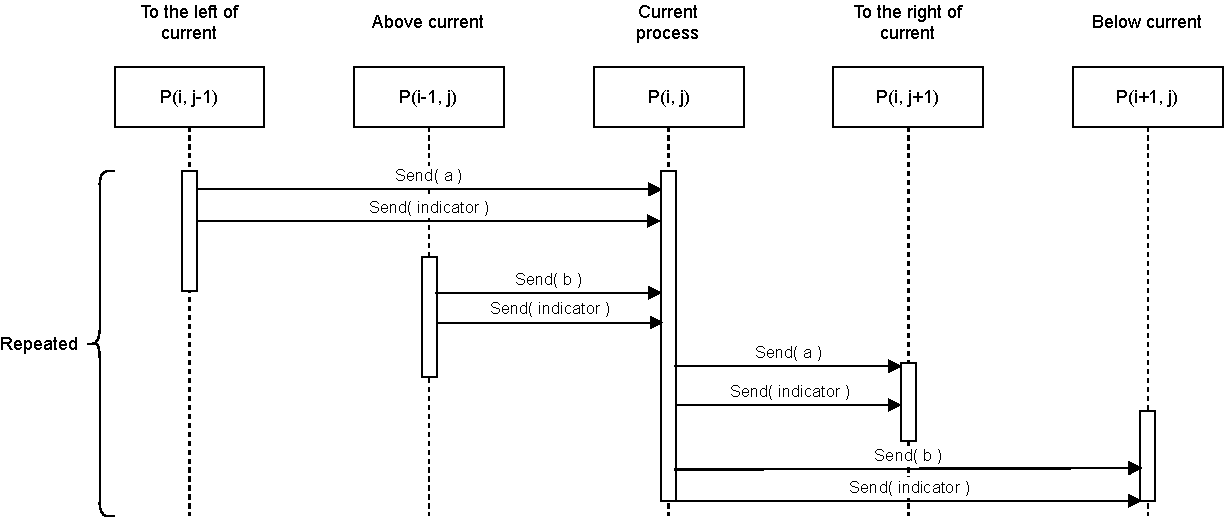
\includegraphics[scale=0.8]{sequence_diagram.pdf}
        \caption{A general representation of the sequence of messages.}
        \label{fig:sequence_diagram}
    \end{figure}

    \subsubsection*{Root}
    This group contains only the root process. It is the only process that reads from
    both files. After reading the inputs, the next iteration of $c$ is computed and
    the input values are propagated into the mesh. It finishes its computations after
    encountering a newline or EOF in the first file.

    \subsubsection*{First row}
    During the first iteration, all processes in this group move to their respective
    initial positions in the second file. This means to the top of the \texttt{rank}-th
    column of matrix $B$. After this these processes read the next value from $B$ and
    wait for the next value from $A$ sent from the process to their left.
    The next iteration of $c$ is computed and the incoming values are propagated into
    the mesh. If there are no more values to be sent, then a message indicating this
    is propagated as well.

    \subsubsection*{First column}
    Similar to the previous group. During the first iteration all processes in this
    group move to their respective positions in the first file, so to
    the $\frac{\texttt{rank}}{\texttt{cols}}$-th row of matrix $A$. After this these
    processes read the next value from $A$ and wait for the next value from $B$ sent
    from theprocess to their top. The next iteration of $c$ is computed and the
    incoming values are propagated into the mesh. If there are no more values
    to be sent, then a message indicating this is propagated as well.

    \subsubsection*{The rest}
    These processes listen to their neighbours for values, as well as to the message
    indicating no more incoming values. The next iteration of $c$ is computed and
    all received messages are propagated further into the mesh. If a message
    indicating the exhaustion of input values is received, the process may finish
    the computation.

\end{document}